% Options for packages loaded elsewhere
\PassOptionsToPackage{unicode}{hyperref}
\PassOptionsToPackage{hyphens}{url}
%
\documentclass[
  ignorenonframetext,
]{beamer}
\usepackage{pgfpages}
\setbeamertemplate{caption}[numbered]
\setbeamertemplate{caption label separator}{: }
\setbeamercolor{caption name}{fg=normal text.fg}
\beamertemplatenavigationsymbolsempty
% Prevent slide breaks in the middle of a paragraph
\widowpenalties 1 10000
\raggedbottom
\setbeamertemplate{part page}{
  \centering
  \begin{beamercolorbox}[sep=16pt,center]{part title}
    \usebeamerfont{part title}\insertpart\par
  \end{beamercolorbox}
}
\setbeamertemplate{section page}{
  \centering
  \begin{beamercolorbox}[sep=12pt,center]{part title}
    \usebeamerfont{section title}\insertsection\par
  \end{beamercolorbox}
}
\setbeamertemplate{subsection page}{
  \centering
  \begin{beamercolorbox}[sep=8pt,center]{part title}
    \usebeamerfont{subsection title}\insertsubsection\par
  \end{beamercolorbox}
}
\AtBeginPart{
  \frame{\partpage}
}
\AtBeginSection{
  \ifbibliography
  \else
    \frame{\sectionpage}
  \fi
}
\AtBeginSubsection{
  \frame{\subsectionpage}
}
\usepackage{amsmath,amssymb}
\usepackage{lmodern}
\usepackage{iftex}
\ifPDFTeX
  \usepackage[T1]{fontenc}
  \usepackage[utf8]{inputenc}
  \usepackage{textcomp} % provide euro and other symbols
\else % if luatex or xetex
  \usepackage{unicode-math}
  \defaultfontfeatures{Scale=MatchLowercase}
  \defaultfontfeatures[\rmfamily]{Ligatures=TeX,Scale=1}
\fi
\usetheme[]{CambridgeUS}
\usefonttheme{structurebold}
% Use upquote if available, for straight quotes in verbatim environments
\IfFileExists{upquote.sty}{\usepackage{upquote}}{}
\IfFileExists{microtype.sty}{% use microtype if available
  \usepackage[]{microtype}
  \UseMicrotypeSet[protrusion]{basicmath} % disable protrusion for tt fonts
}{}
\makeatletter
\@ifundefined{KOMAClassName}{% if non-KOMA class
  \IfFileExists{parskip.sty}{%
    \usepackage{parskip}
  }{% else
    \setlength{\parindent}{0pt}
    \setlength{\parskip}{6pt plus 2pt minus 1pt}}
}{% if KOMA class
  \KOMAoptions{parskip=half}}
\makeatother
\usepackage{xcolor}
\newif\ifbibliography
\usepackage{color}
\usepackage{fancyvrb}
\newcommand{\VerbBar}{|}
\newcommand{\VERB}{\Verb[commandchars=\\\{\}]}
\DefineVerbatimEnvironment{Highlighting}{Verbatim}{commandchars=\\\{\}}
% Add ',fontsize=\small' for more characters per line
\usepackage{framed}
\definecolor{shadecolor}{RGB}{248,248,248}
\newenvironment{Shaded}{\begin{snugshade}}{\end{snugshade}}
\newcommand{\AlertTok}[1]{\textcolor[rgb]{0.94,0.16,0.16}{#1}}
\newcommand{\AnnotationTok}[1]{\textcolor[rgb]{0.56,0.35,0.01}{\textbf{\textit{#1}}}}
\newcommand{\AttributeTok}[1]{\textcolor[rgb]{0.77,0.63,0.00}{#1}}
\newcommand{\BaseNTok}[1]{\textcolor[rgb]{0.00,0.00,0.81}{#1}}
\newcommand{\BuiltInTok}[1]{#1}
\newcommand{\CharTok}[1]{\textcolor[rgb]{0.31,0.60,0.02}{#1}}
\newcommand{\CommentTok}[1]{\textcolor[rgb]{0.56,0.35,0.01}{\textit{#1}}}
\newcommand{\CommentVarTok}[1]{\textcolor[rgb]{0.56,0.35,0.01}{\textbf{\textit{#1}}}}
\newcommand{\ConstantTok}[1]{\textcolor[rgb]{0.00,0.00,0.00}{#1}}
\newcommand{\ControlFlowTok}[1]{\textcolor[rgb]{0.13,0.29,0.53}{\textbf{#1}}}
\newcommand{\DataTypeTok}[1]{\textcolor[rgb]{0.13,0.29,0.53}{#1}}
\newcommand{\DecValTok}[1]{\textcolor[rgb]{0.00,0.00,0.81}{#1}}
\newcommand{\DocumentationTok}[1]{\textcolor[rgb]{0.56,0.35,0.01}{\textbf{\textit{#1}}}}
\newcommand{\ErrorTok}[1]{\textcolor[rgb]{0.64,0.00,0.00}{\textbf{#1}}}
\newcommand{\ExtensionTok}[1]{#1}
\newcommand{\FloatTok}[1]{\textcolor[rgb]{0.00,0.00,0.81}{#1}}
\newcommand{\FunctionTok}[1]{\textcolor[rgb]{0.00,0.00,0.00}{#1}}
\newcommand{\ImportTok}[1]{#1}
\newcommand{\InformationTok}[1]{\textcolor[rgb]{0.56,0.35,0.01}{\textbf{\textit{#1}}}}
\newcommand{\KeywordTok}[1]{\textcolor[rgb]{0.13,0.29,0.53}{\textbf{#1}}}
\newcommand{\NormalTok}[1]{#1}
\newcommand{\OperatorTok}[1]{\textcolor[rgb]{0.81,0.36,0.00}{\textbf{#1}}}
\newcommand{\OtherTok}[1]{\textcolor[rgb]{0.56,0.35,0.01}{#1}}
\newcommand{\PreprocessorTok}[1]{\textcolor[rgb]{0.56,0.35,0.01}{\textit{#1}}}
\newcommand{\RegionMarkerTok}[1]{#1}
\newcommand{\SpecialCharTok}[1]{\textcolor[rgb]{0.00,0.00,0.00}{#1}}
\newcommand{\SpecialStringTok}[1]{\textcolor[rgb]{0.31,0.60,0.02}{#1}}
\newcommand{\StringTok}[1]{\textcolor[rgb]{0.31,0.60,0.02}{#1}}
\newcommand{\VariableTok}[1]{\textcolor[rgb]{0.00,0.00,0.00}{#1}}
\newcommand{\VerbatimStringTok}[1]{\textcolor[rgb]{0.31,0.60,0.02}{#1}}
\newcommand{\WarningTok}[1]{\textcolor[rgb]{0.56,0.35,0.01}{\textbf{\textit{#1}}}}
\usepackage{graphicx}
\makeatletter
\def\maxwidth{\ifdim\Gin@nat@width>\linewidth\linewidth\else\Gin@nat@width\fi}
\def\maxheight{\ifdim\Gin@nat@height>\textheight\textheight\else\Gin@nat@height\fi}
\makeatother
% Scale images if necessary, so that they will not overflow the page
% margins by default, and it is still possible to overwrite the defaults
% using explicit options in \includegraphics[width, height, ...]{}
\setkeys{Gin}{width=\maxwidth,height=\maxheight,keepaspectratio}
% Set default figure placement to htbp
\makeatletter
\def\fps@figure{htbp}
\makeatother
\setlength{\emergencystretch}{3em} % prevent overfull lines
\providecommand{\tightlist}{%
  \setlength{\itemsep}{0pt}\setlength{\parskip}{0pt}}
\setcounter{secnumdepth}{-\maxdimen} % remove section numbering
\definecolor{color1}{rgb}{0.0,0.18,0.39}
\definecolor{color2}{HTML}{050A2A}
\definecolor{color3}{HTML}{232C6A}
\definecolor{color4}{HTML}{5D6BB3}
\setbeamercolor{background}{fg=white, bg=color2}
\setbeamercolor{palette primary}{fg=white, bg=color2}
\setbeamercolor{palette secondary}{fg=white, bg=color3}
\setbeamercolor{palette tertiary}{fg=white, bg=color4}
\setbeamercolor{frametitle}{fg=white, bg=color2}
\setbeamercolor{title}{fg=color2}
\usefonttheme{professionalfonts}
\setbeamerfont{title}{size=\huge}
\setbeamerfont{subtitle}{size=\Large}
\setbeamerfont{author}{size=\small}
\setbeamerfont{date}{size=\large}
\ifLuaTeX
  \usepackage{selnolig}  % disable illegal ligatures
\fi
\IfFileExists{bookmark.sty}{\usepackage{bookmark}}{\usepackage{hyperref}}
\IfFileExists{xurl.sty}{\usepackage{xurl}}{} % add URL line breaks if available
\urlstyle{same} % disable monospaced font for URLs
\hypersetup{
  pdftitle={PSTAT 126},
  pdfauthor={Laura Baracaldo \& Rodrigo Targino},
  hidelinks,
  pdfcreator={LaTeX via pandoc}}

\title{PSTAT 126}
\subtitle{Regression Analysis}
\author{Laura Baracaldo \& Rodrigo Targino}
\date{Lecture 1\\
Introduction to Linear Models}

\begin{document}
\frame{\titlepage}

\begin{frame}{Introduction}
\protect\hypertarget{introduction}{}
Regression Analysis: Statistical method that allows the exploration of
the relationship between two or more variables.
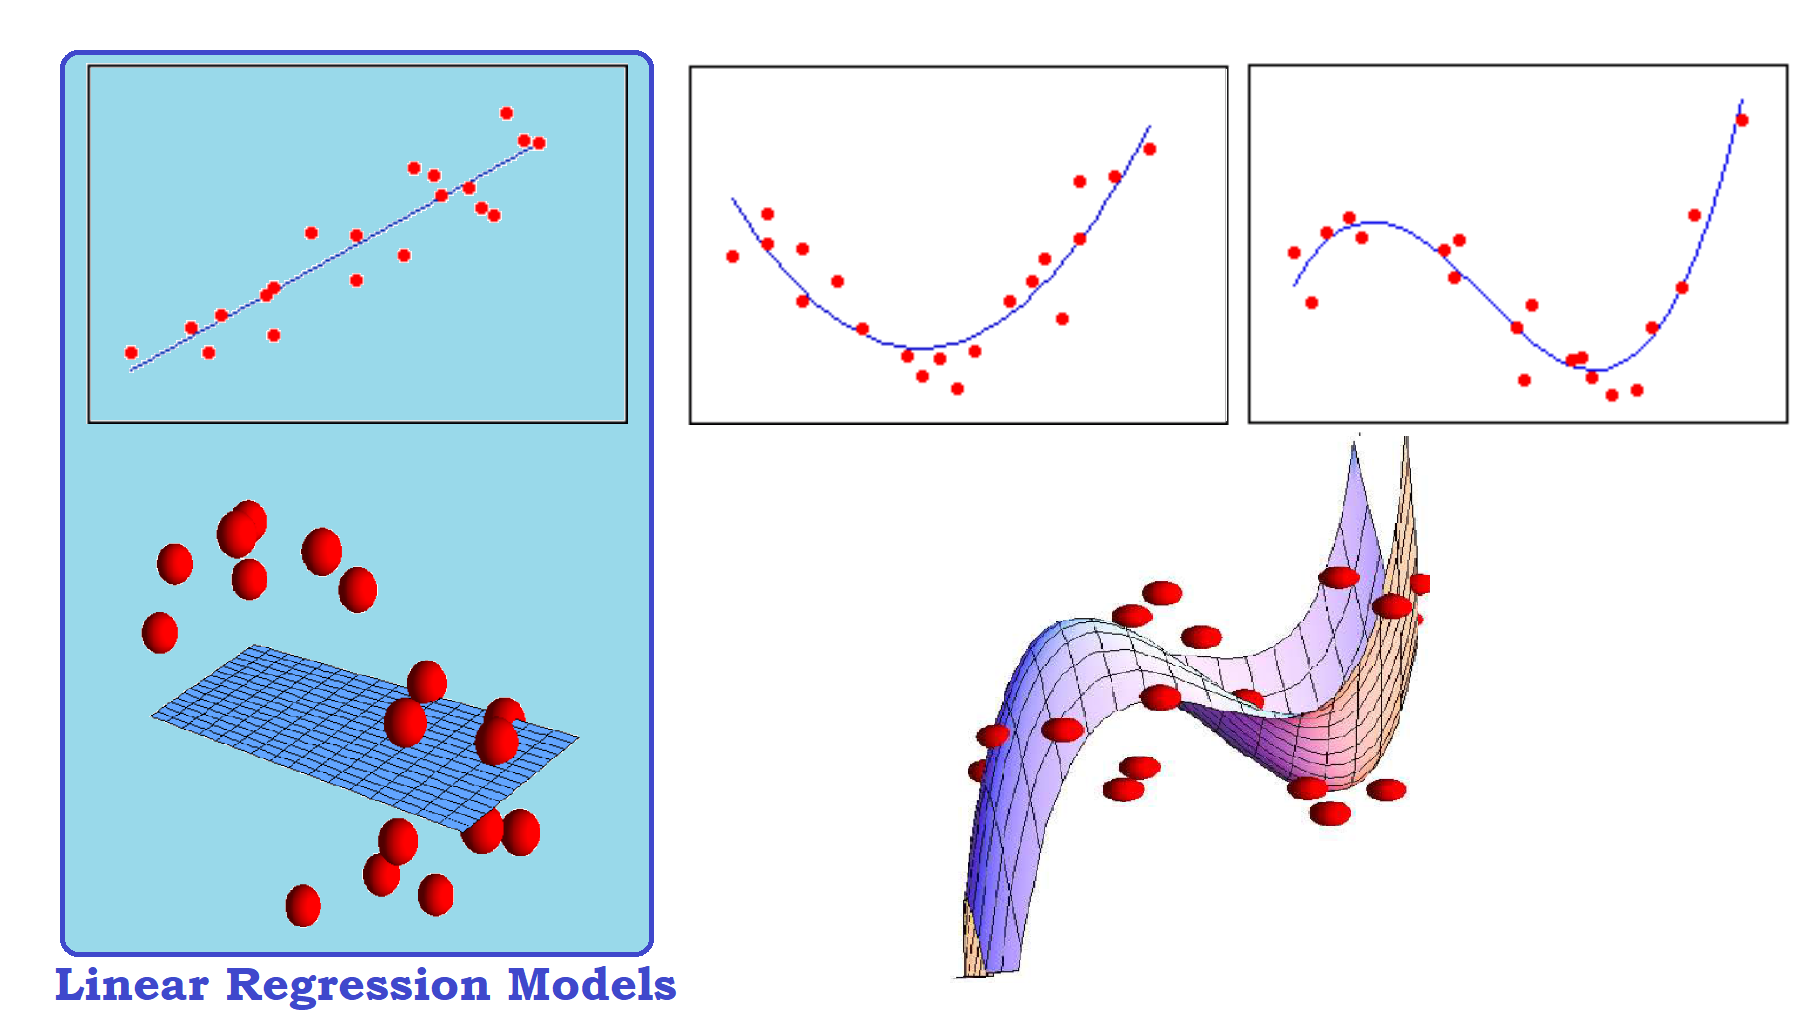
\includegraphics[width=0.8\textwidth,height=\textheight]{image1.png}\\
\end{frame}

\begin{frame}{Introduction}
\protect\hypertarget{introduction-1}{}
\begin{itemize}
\tightlist
\item
  \(Y:\) Response, outcome, output, dependent variable.
\item
  \((X_1, ...X_p)^T:\) vector of predictors, inputs, independent or
  explanatory variables.
\end{itemize}

Goals:

\begin{enumerate}
\tightlist
\item
  Prediction of future or unmeasured responses given values of the
  predictors.
\item
  Assessment of the effect/relationship between explanatory variables
  and response. Existence of causality?
\end{enumerate}
\end{frame}

\begin{frame}[fragile]{Cars example}
\protect\hypertarget{cars-example}{}
\href{./cars.html}{Link to help}

\(X:\) Speed \(\qquad Y:\) Distance

\begin{Shaded}
\begin{Highlighting}[]
\FunctionTok{par}\NormalTok{(}\AttributeTok{mar=}\FunctionTok{c}\NormalTok{(}\DecValTok{3}\NormalTok{,}\DecValTok{4}\NormalTok{,}\FloatTok{0.5}\NormalTok{,}\DecValTok{1}\NormalTok{))}
\FunctionTok{plot}\NormalTok{(cars, }\AttributeTok{pch=}\DecValTok{18}\NormalTok{)}
\end{Highlighting}
\end{Shaded}

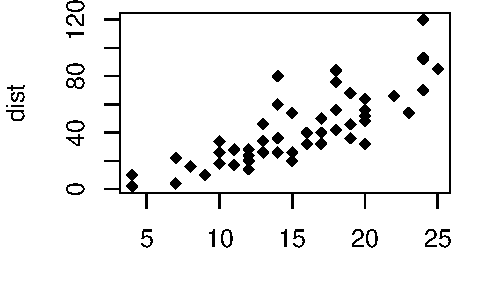
\includegraphics{Lec1_files/figure-beamer/cars1-1.pdf}
\end{frame}

\begin{frame}[fragile]{Cars example}
\protect\hypertarget{cars-example-1}{}
\(X:\) Speed \(\qquad Y:\) Distance

\begin{Shaded}
\begin{Highlighting}[]
\FunctionTok{par}\NormalTok{(}\AttributeTok{mar=}\FunctionTok{c}\NormalTok{(}\DecValTok{3}\NormalTok{,}\DecValTok{4}\NormalTok{,}\FloatTok{0.5}\NormalTok{,}\DecValTok{1}\NormalTok{))}
\FunctionTok{plot}\NormalTok{(cars, }\AttributeTok{pch=}\DecValTok{18}\NormalTok{)}
\FunctionTok{abline}\NormalTok{(}\FunctionTok{lm}\NormalTok{( dist }\SpecialCharTok{\textasciitilde{}}\NormalTok{ speed, }\AttributeTok{data=}\NormalTok{cars), }\AttributeTok{col=}\StringTok{"blue"}\NormalTok{)}
\end{Highlighting}
\end{Shaded}

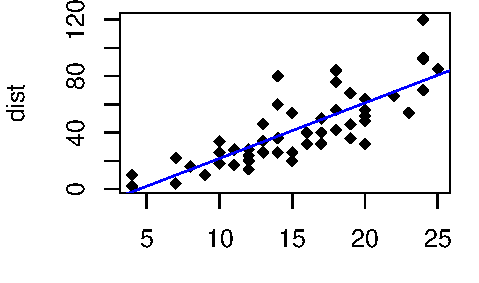
\includegraphics{Lec1_files/figure-beamer/cars2-1.pdf}
\end{frame}

\begin{frame}[fragile]{Cheddar example}
\protect\hypertarget{cheddar-example}{}
\begin{verbatim}
## Warning: package 'faraway' was built under R version 4.2.2
\end{verbatim}

\href{./cheddar.html}{Link to help}

\(X:\) Hydrogen sulfide concentration \(\qquad Y:\) Taste score

\begin{Shaded}
\begin{Highlighting}[]
\FunctionTok{library}\NormalTok{(faraway)}
\FunctionTok{par}\NormalTok{(}\AttributeTok{mar=}\FunctionTok{c}\NormalTok{(}\DecValTok{3}\NormalTok{,}\DecValTok{4}\NormalTok{,}\FloatTok{0.5}\NormalTok{,}\DecValTok{1}\NormalTok{))}
\FunctionTok{plot}\NormalTok{(cheddar}\SpecialCharTok{$}\NormalTok{H2S, cheddar}\SpecialCharTok{$}\NormalTok{taste, }\AttributeTok{pch=}\DecValTok{18}\NormalTok{)}
\end{Highlighting}
\end{Shaded}

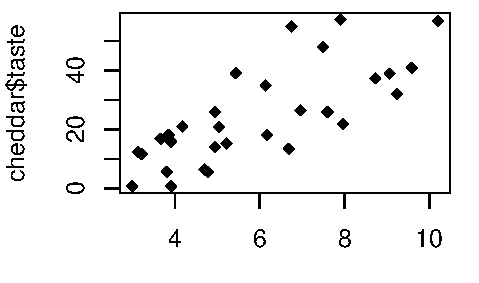
\includegraphics{Lec1_files/figure-beamer/che1-1.pdf}
\end{frame}

\begin{frame}[fragile]{Cheddar example}
\protect\hypertarget{cheddar-example-1}{}
\(X:\) Hydrogen sulfide concentration \(\qquad Y:\) Taste score

\begin{Shaded}
\begin{Highlighting}[]
\FunctionTok{library}\NormalTok{(faraway)}
\FunctionTok{par}\NormalTok{(}\AttributeTok{mar=}\FunctionTok{c}\NormalTok{(}\DecValTok{3}\NormalTok{,}\DecValTok{4}\NormalTok{,}\FloatTok{0.5}\NormalTok{,}\DecValTok{1}\NormalTok{))}
\FunctionTok{plot}\NormalTok{(cheddar}\SpecialCharTok{$}\NormalTok{H2S, cheddar}\SpecialCharTok{$}\NormalTok{taste, }\AttributeTok{pch=}\DecValTok{18}\NormalTok{)}
\FunctionTok{abline}\NormalTok{(}\FunctionTok{lm}\NormalTok{( taste }\SpecialCharTok{\textasciitilde{}}\NormalTok{ H2S, }\AttributeTok{data=}\NormalTok{cheddar), }\AttributeTok{col=}\StringTok{"blue"}\NormalTok{)}
\end{Highlighting}
\end{Shaded}

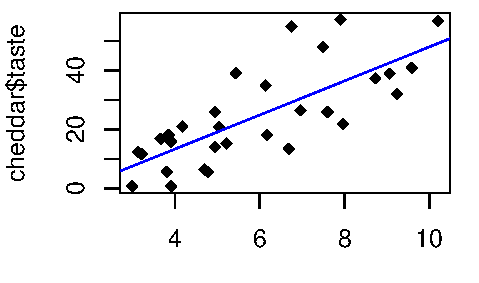
\includegraphics{Lec1_files/figure-beamer/che2-1.pdf}
\end{frame}

\begin{frame}[fragile]{Pressure example}
\protect\hypertarget{pressure-example}{}
\href{./pressure.html}{Link to help}

\(X:\) Temperature \(\qquad Y:\) Pressure

\begin{Shaded}
\begin{Highlighting}[]
\FunctionTok{par}\NormalTok{(}\AttributeTok{mar=}\FunctionTok{c}\NormalTok{(}\DecValTok{3}\NormalTok{,}\DecValTok{4}\NormalTok{,}\FloatTok{0.5}\NormalTok{,}\DecValTok{1}\NormalTok{))}
\FunctionTok{plot}\NormalTok{(pressure, }\AttributeTok{pch=}\DecValTok{18}\NormalTok{)}
\end{Highlighting}
\end{Shaded}

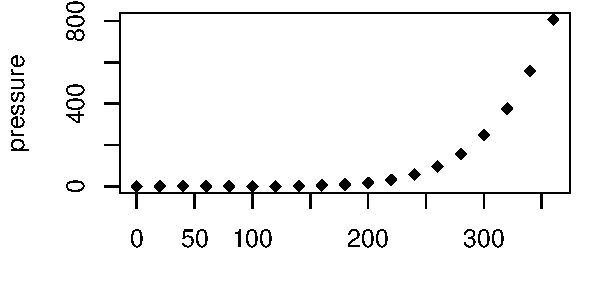
\includegraphics{Lec1_files/figure-beamer/pre1-1.pdf}
\end{frame}

\begin{frame}[fragile]{Pressure example}
\protect\hypertarget{pressure-example-1}{}
\(X:\) Temperature \(\qquad Y:\) Pressure

\begin{Shaded}
\begin{Highlighting}[]
\FunctionTok{par}\NormalTok{(}\AttributeTok{mar=}\FunctionTok{c}\NormalTok{(}\DecValTok{3}\NormalTok{,}\DecValTok{4}\NormalTok{,}\FloatTok{0.5}\NormalTok{,}\DecValTok{1}\NormalTok{))}
\FunctionTok{plot}\NormalTok{(pressure, }\AttributeTok{pch=}\DecValTok{18}\NormalTok{)}
\FunctionTok{abline}\NormalTok{(}\FunctionTok{lm}\NormalTok{( pressure }\SpecialCharTok{\textasciitilde{}}\NormalTok{ temperature, }\AttributeTok{data=}\NormalTok{pressure), }\AttributeTok{col=}\StringTok{"red"}\NormalTok{)}
\end{Highlighting}
\end{Shaded}

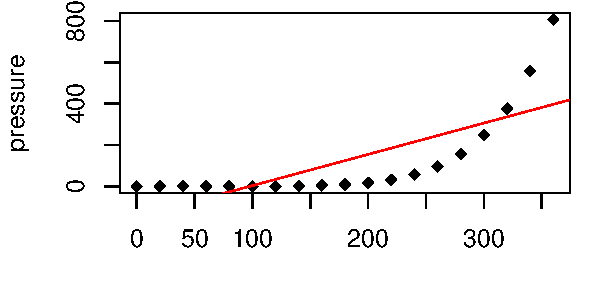
\includegraphics{Lec1_files/figure-beamer/pre2-1.pdf}
\end{frame}

\begin{frame}{Regression vs Classification}
\protect\hypertarget{regression-vs-classification}{}
\begin{itemize}
\tightlist
\item
  Regression: \(Y\) is continuous. Numerical values (e.g.~price, blood
  pressure, confirmed COVID-19 cases).
\item
  Classification \(Y\) discrete labels. Categorical values.
  (e.g.~survived/died, digit 0-9, if Bitcoin price is going up
  tomorrow).
\end{itemize}

\centering

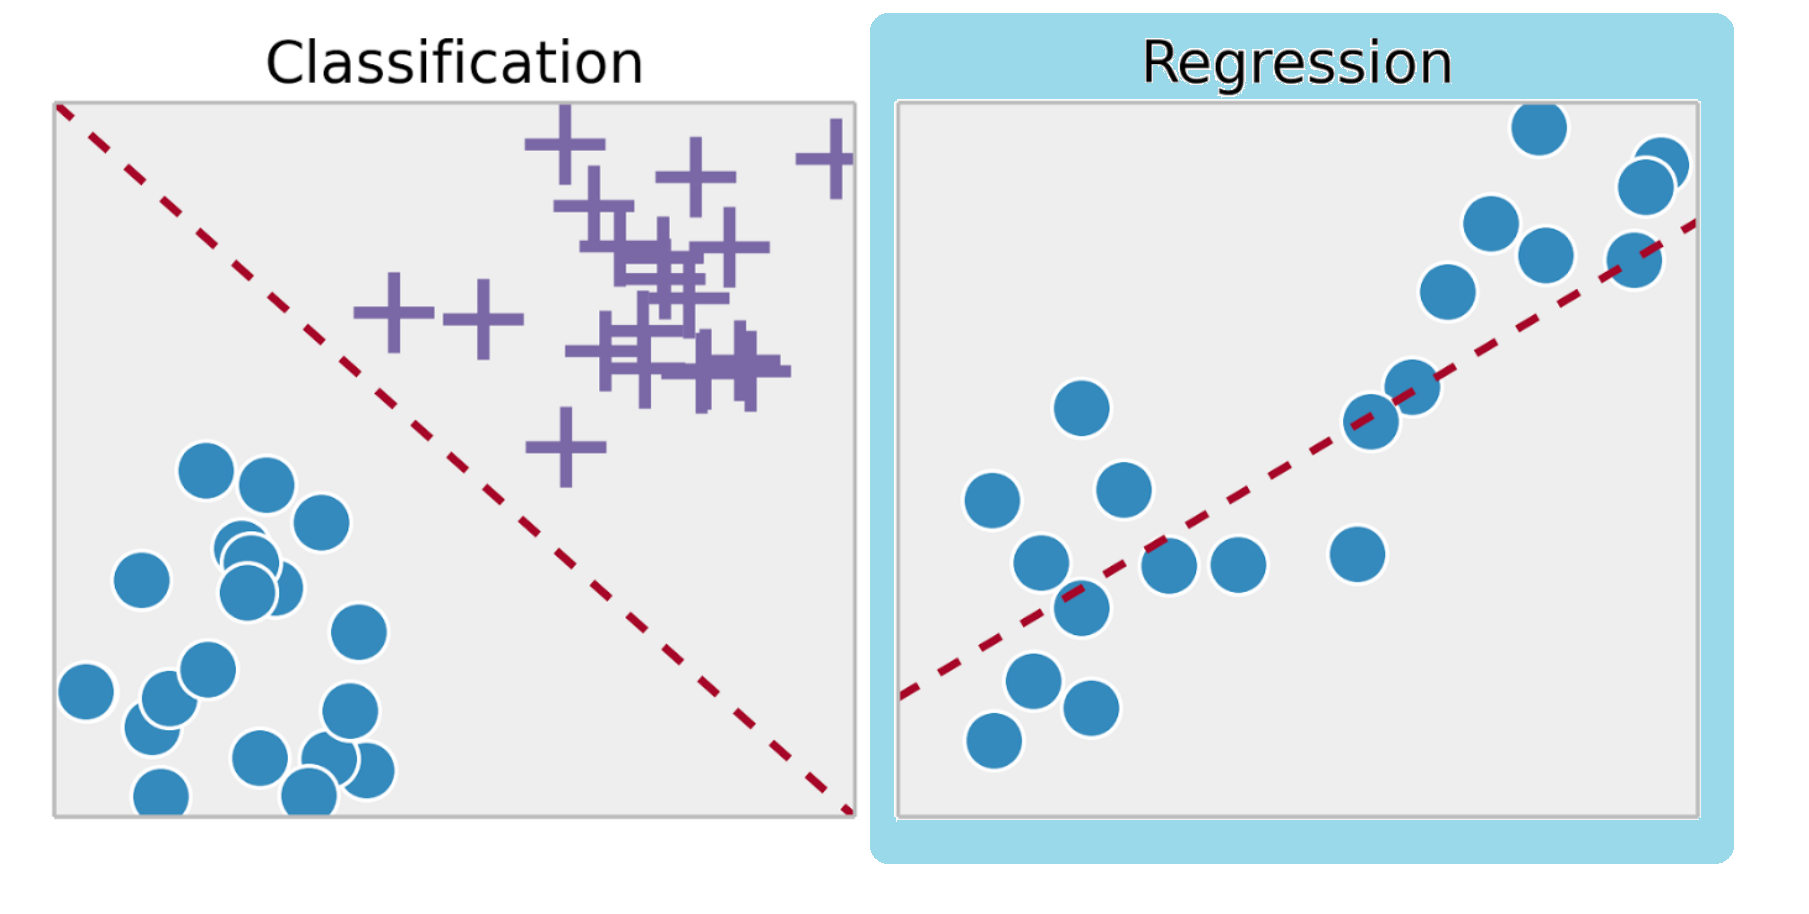
\includegraphics[width=0.6\textwidth,height=\textheight]{image2.png}\\
\end{frame}

\begin{frame}{General Workflow}
\protect\hypertarget{general-workflow}{}
\centering

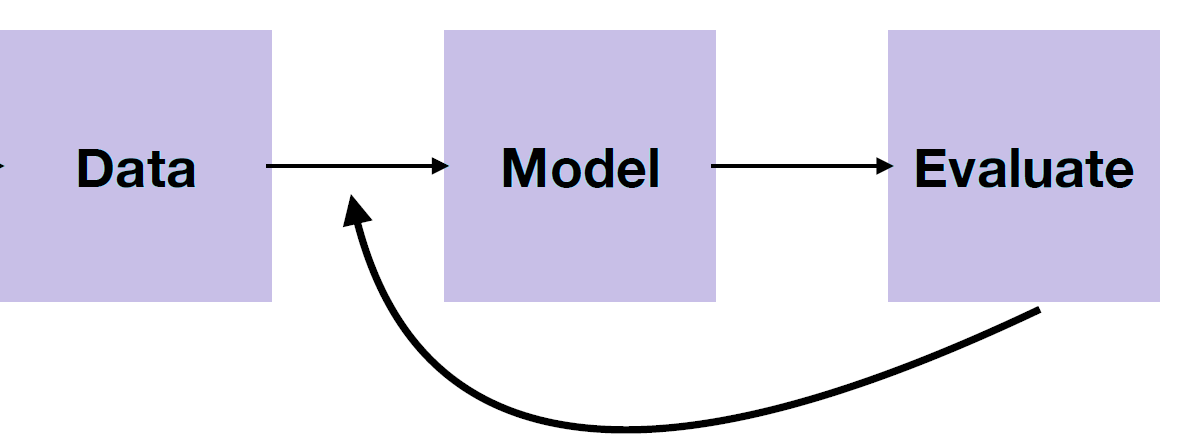
\includegraphics[width=0.6\textwidth,height=\textheight]{image3.png}\\
1. Data: We collect data for all \(n\) subjects in the study, and
identify \(Y\) and \(X\):

\[ Y = \begin{bmatrix}
           y_{1} \\
            \\
                  \\
         \end{bmatrix}  \qquad \qquad  X = \begin{bmatrix}
           x_{11}& x_{12} &...&x_{1p}\\
          &&&\\
           & & &
         \end{bmatrix} \]
\end{frame}

\begin{frame}{General Workflow}
\protect\hypertarget{general-workflow-1}{}
\centering

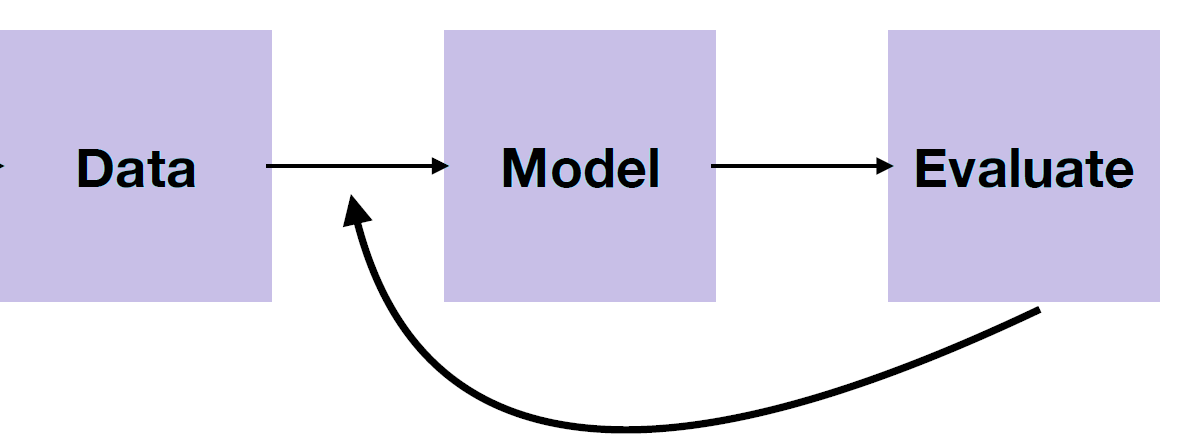
\includegraphics[width=0.6\textwidth,height=\textheight]{image3.png}\\
1. Data: We collect data for all \(n\) subjects in the study, and
identify \(Y\) and \(X\):

\[ Y = \begin{bmatrix}
           y_{1} \\
           y_{2} \\
                  \\
         \end{bmatrix}  \qquad \qquad  X = \begin{bmatrix}
           x_{11}& x_{12} &...&x_{1p}\\
           x_{21}& x_{22} &...&x_{2p} \\
           & & &
         \end{bmatrix} \]
\end{frame}

\begin{frame}{General Workflow}
\protect\hypertarget{general-workflow-2}{}
\centering

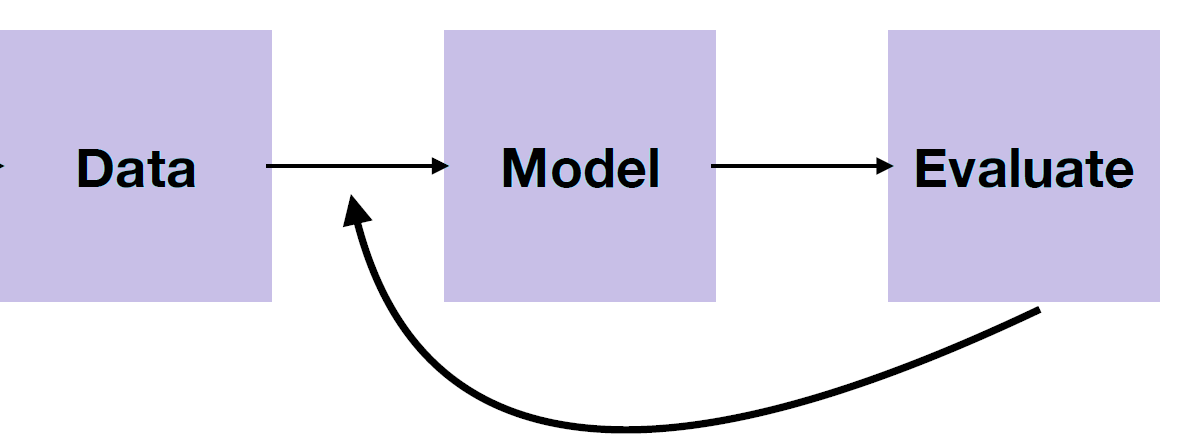
\includegraphics[width=0.6\textwidth,height=\textheight]{image3.png}\\
1. Data: We collect data for all \(n\) subjects in the study, and
identify \(Y\) and \(X\):

\[ Y = \begin{bmatrix}
           y_{1} \\
           y_{2} \\
           \vdots \\
           y_{n}
         \end{bmatrix}  \qquad \qquad  X = \begin{bmatrix}
           x_{11}& x_{12} &...&x_{1p}\\
           x_{21}& x_{22} &...&x_{2p} \\
           \vdots &\vdots& ...&\vdots\\
           x_{n1}& x_{n2} &...&x_{np}
         \end{bmatrix} \]

\begin{itemize}
\tightlist
\item
  \(Y \in \mathbb{R}^{n}\), \(X \in \mathbb{R}^{n \times p}\)
\end{itemize}
\end{frame}

\begin{frame}{Regression Model}
\protect\hypertarget{regression-model}{}
\[Y= f(X_1, X_2, ...X_p) + \epsilon\]

\begin{itemize}
\tightlist
\item
  \(\epsilon:\) Error/noise
\item
  \(f\) is unknown and must be learned from observations
  \((Y, X_1, ..., X_p)\)
\item
  Questions about \(f\). Continuous? Smooth?
\item
  \(f\) must be restricted. In this course: We assume \(f\) is linear.
\end{itemize}
\end{frame}

\begin{frame}{Linear Regression Model}
\protect\hypertarget{linear-regression-model}{}
We assume the response is written as linear representation of
predictors:

\[Y = \beta_0 + \beta_1X_1+...\beta_pX_p + \epsilon\]

\begin{itemize}
\tightlist
\item
  \textbf{Estimation:} The goal is to estimate unknown parameters
  \(\beta_0, \beta_1, ...\beta_p\).
\end{itemize}
\end{frame}

\begin{frame}{Linear Regression Model}
\protect\hypertarget{linear-regression-model-1}{}
\begin{itemize}
\item
  \textbf{Linear:}
  \[Y = \beta_0 + \beta_1 log(X_1)+...\beta_pX_p^2 + \epsilon = \beta_0 + \beta_1 W_1+...\beta_pW_p + \epsilon \]
\item
  \textbf{NOT Linear:}
  \[Y = \beta_0 +  X_1^{\beta_1}+...\beta_pX_p + \epsilon\]
\end{itemize}
\end{frame}

\begin{frame}{Matrix Representation}
\protect\hypertarget{matrix-representation}{}
\[\begin{bmatrix}
           y_{1} \\
           y_{2} \\
           \vdots \\
           y_{n}
         \end{bmatrix}  = \begin{bmatrix}
           1& x_{11} &...&x_{1p}\\
           1& x_{21} &...&x_{2p} \\
           \vdots &\vdots& ...&\vdots\\
           1& x_{n1} &...&x_{np}
         \end{bmatrix}  \begin{bmatrix}
           \beta_{0} \\
           \beta_{1} \\
           \vdots \\
           \beta_{p}
         \end{bmatrix} +  \begin{bmatrix}
           \epsilon_{1} \\
           \epsilon_{2} \\
           \vdots \\
           \epsilon_{n}
         \end{bmatrix}\]

\[ Y = X\beta + \epsilon\]
\end{frame}

\begin{frame}{Model Assessment}
\protect\hypertarget{model-assessment}{}
\begin{enumerate}
\tightlist
\item
  Prediction: accurately predict future response given predictors.
\item
  Inference: assess the quality of our predictions and (or) estimation.
\item
  Diagnostics: what if the linear model assumptions go wrong? how can we
  tell?
\item
  Model selection: find the ``best'' linear model for response given
  predictors.
\end{enumerate}
\end{frame}

\begin{frame}{Next\ldots{}}
\protect\hypertarget{next}{}
\begin{itemize}
\tightlist
\item
  Set up your R working environment.
\item
  Lab sessions and TAs' office hours start next week.
\item
  Office hours:

  \begin{itemize}
  \tightlist
  \item
    Prof.~Baracaldo: TBD
  \item
    Prof.~Targino: Fridays 1.30pm - 3.30pm OG1230 or on Zoom
    \url{https://fgv-br.zoom.us/j/95030256507}
  \end{itemize}
\end{itemize}
\end{frame}

\end{document}
